\chapter{EXPERIMENTAL OPTIMIZATION OF PLASMA-LIQUID INTERACTIONS: VHF SOURCE}
\label{chap:expt_opt}

In a quest to optimize interaction between water and plasmas generated with the source described in \cite{byrns2012vhf}, several geometric configurations have been iterated over. These iterations are described in the following sections.

\section{Base Set-up}

The experimental set-up shown in \cref{fig:batch_scheme} is known as the ``batch'' set-up. It was the first plasma-water configuration explored by the group. Originally it was intended for degradation of perfluorinated compounds like perfluorooctanesulfonic acid (PFOS) and perfluorootanoic acid (PFOA). It turned out that the batch configuration was unable to degrade these persistent chemicals; however, in the process it was discovered that the configuration generated large amounts of NO$_x$, mostly NO$_3^-$, in the aqueous phase. Generation of nitrogen and oxygen species (RONS) in solution by plasmas is now a well-known phenomenon in the plasma-liquid community; however, at the time it was a novel discovery for our group. Recognizing that aqueous nitrogen, specifically NO$_3^-$, is a key component in fertilizer, we were motivated to begin a study in collaboration with the horticulture department of plant fertilization using plasma activated water (PAW). This study is outlined in \cref{sec:fertigation}. Later, the batch configuration was used in exploration of dioxane degradation; this is discussed in \cref{sec:dioxane}.

Depending on the application, delivered power to the plasma for the batch configuration ranged between 350 and 1000 W. Many different gases were used, including air, argon, helium, nitrogen, and carbon dioxide. Gas flow rates ranged from 2-5 standard cubic feet per minute. The gap distance between the powered electrode and the water surface ranged from a few milimeters to a couple centimeters, with larger gap distances typically used in combination with larger gas flow rates in order to avoid splashing of the electrode and extinguishing of the plasma. Water treatment volumes ranged from 100-500 mL for persistent chemical studies up to several liters for PAW generation in the fertigation experiments.

\begin{figure}[htbp]
  \centering
  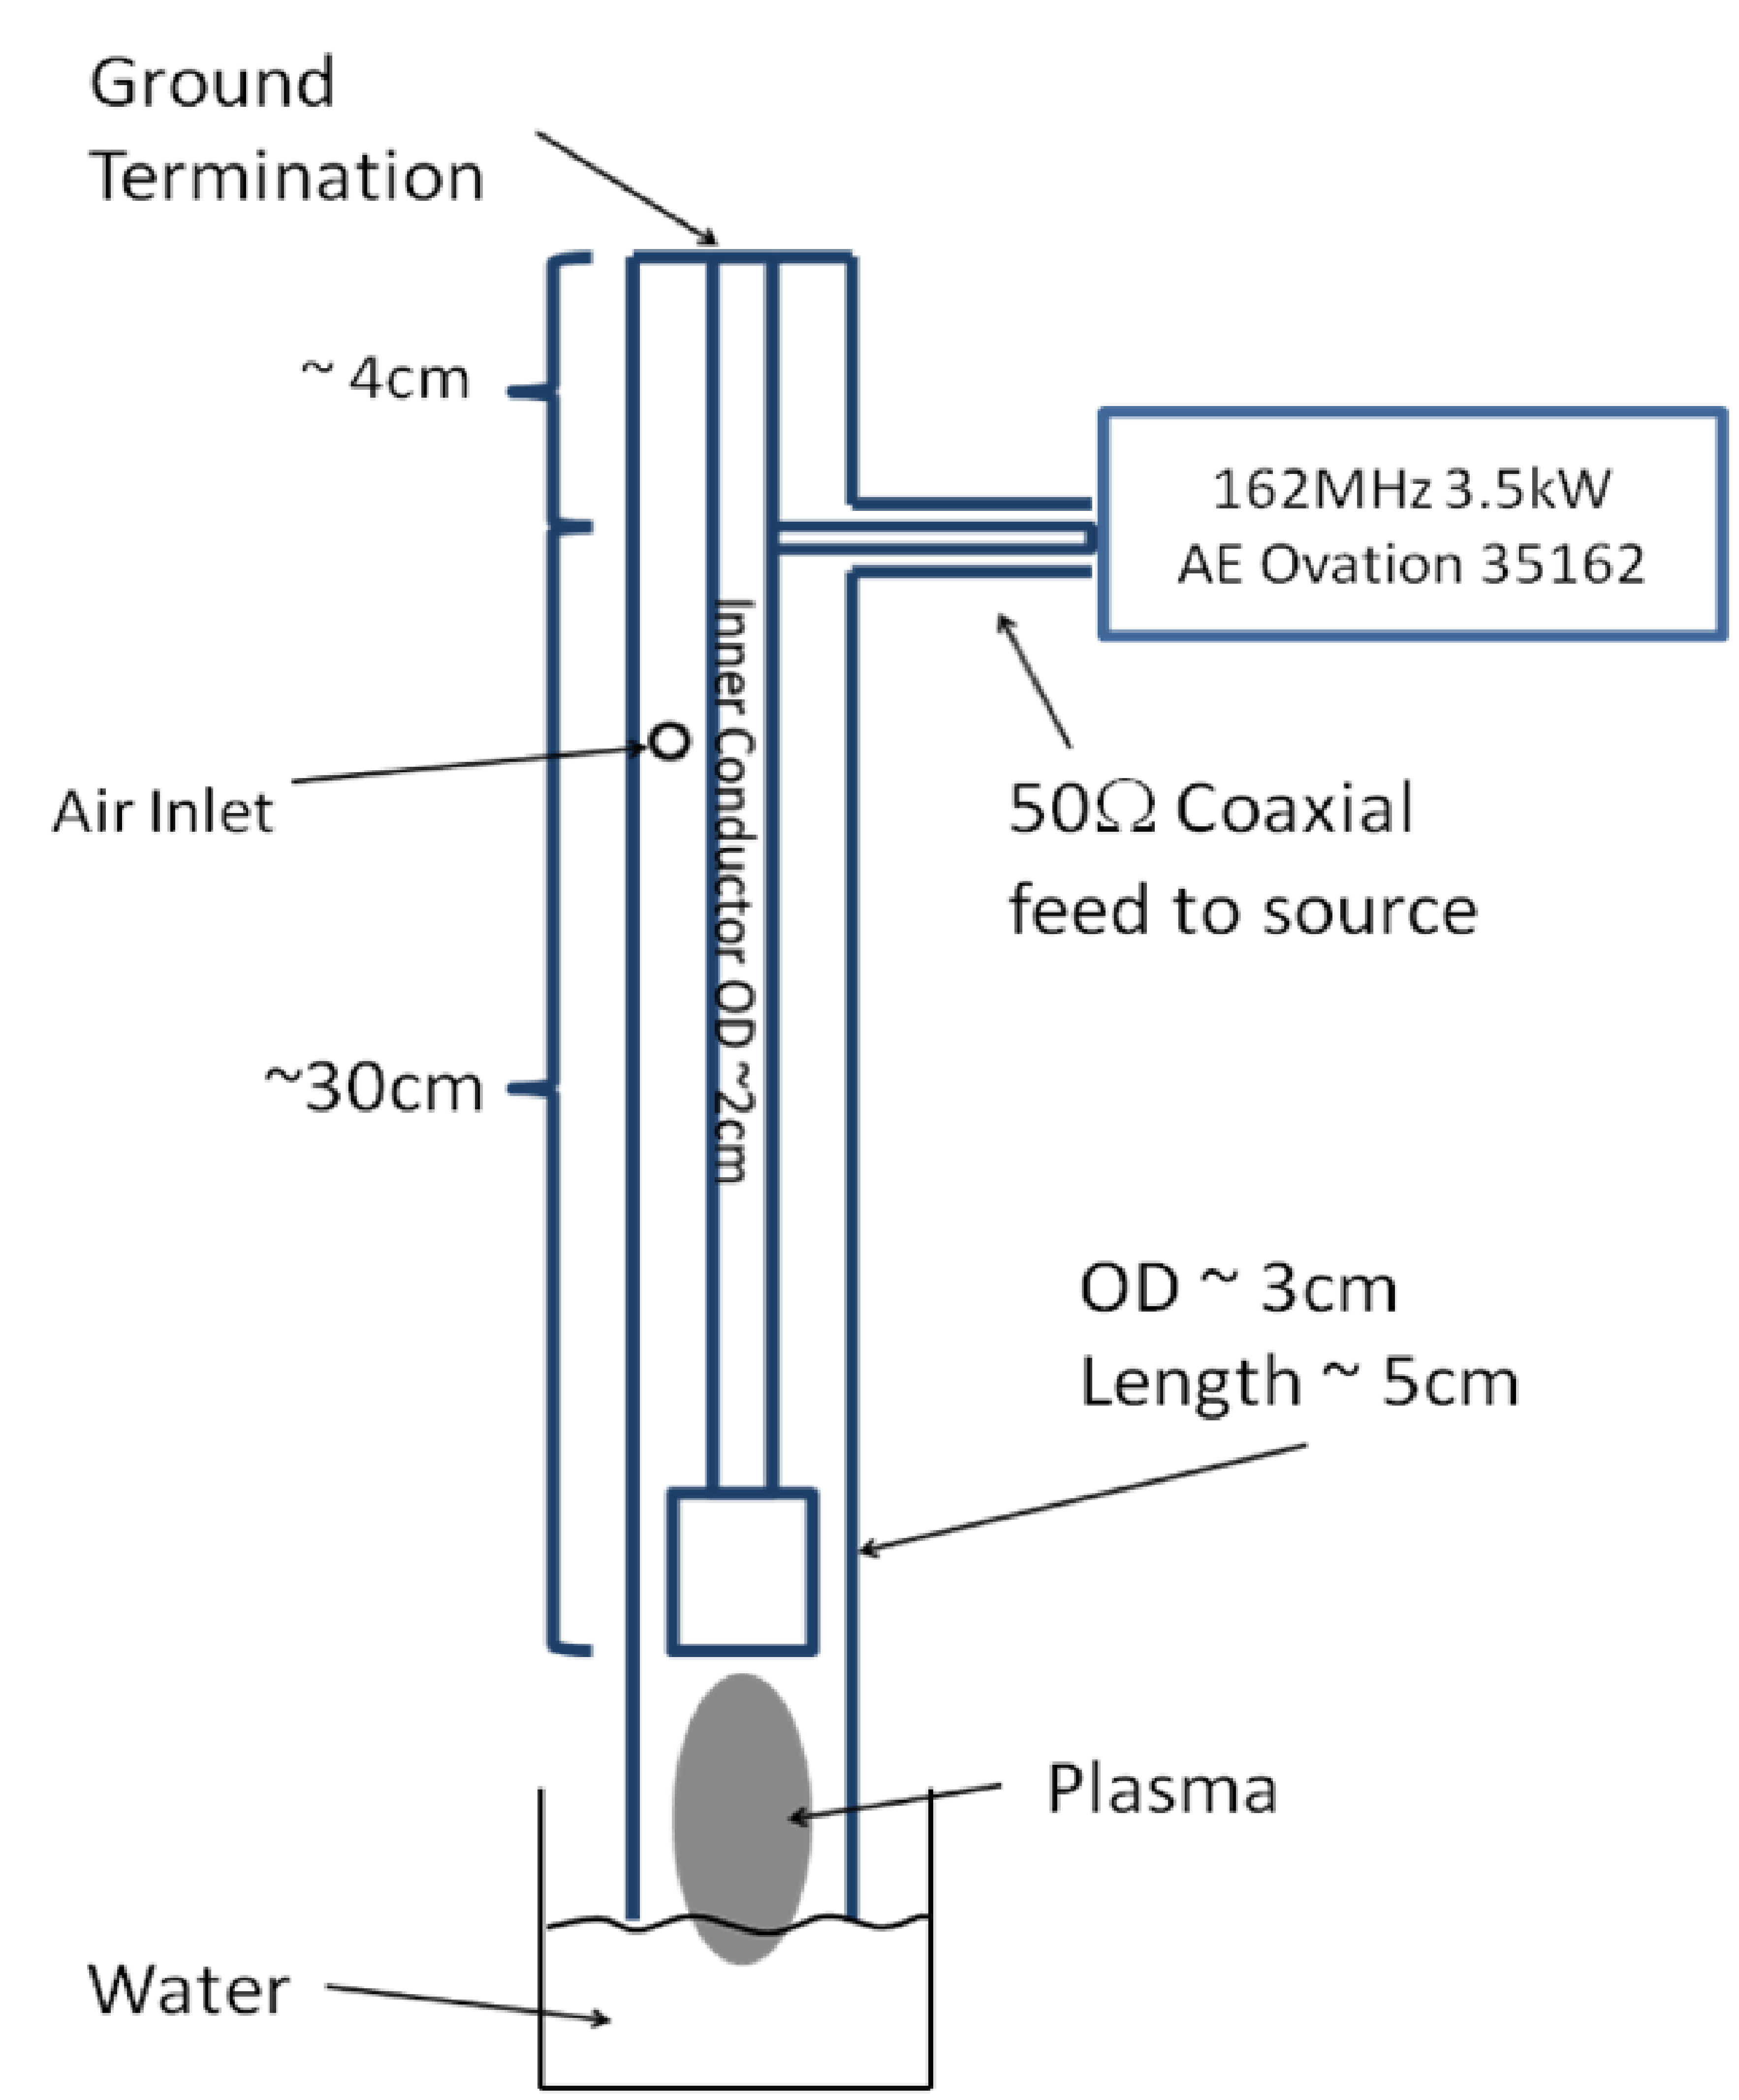
\includegraphics[width=0.9\textwidth]{Figure1_word.pdf}
  \caption{Schematic of the atmospheric plasma source and batch water treatment set-up}
  \label{fig:batch_scheme}
\end{figure}

\section{Spray-through Design}

One way we thought to increase plasma-water interaction was to directly introduce water droplets into the active plasma region. We hypothesized that there were two good reasons for doing this. Firstly, it was reasoned that water droplets passing through the core of the plasma as opposed to the edge or afterglow would be exposed to greater densities of electrons, ions, and reactive radical species. Secondly, by breaking the water volume into droplets, the surface-to-volume ratio would be increased, increasing the rate of mass transfer of plasma species into the aqueous phase. Two different configurations were used to explore these concepts; they are outlined in the following subsections.

\subsection{Spray Bottle}
\label{sec:spray_bottle}

The easiest way to achieve a droplet configuration was to take the batch set-up (see \cref{fig:batch_scheme}) and remove the beaker of water under the coaxial plasma source. Then after turning the plasma on, a greenhouse sprayer was used to pass droplets radially through the plasma; a beaker is used to catch the droplets after passage through the plasma. A summary of the configuration is shown in \cref{fig:spray_scheme}.

\begin{figure}[htbp]
  \centering
  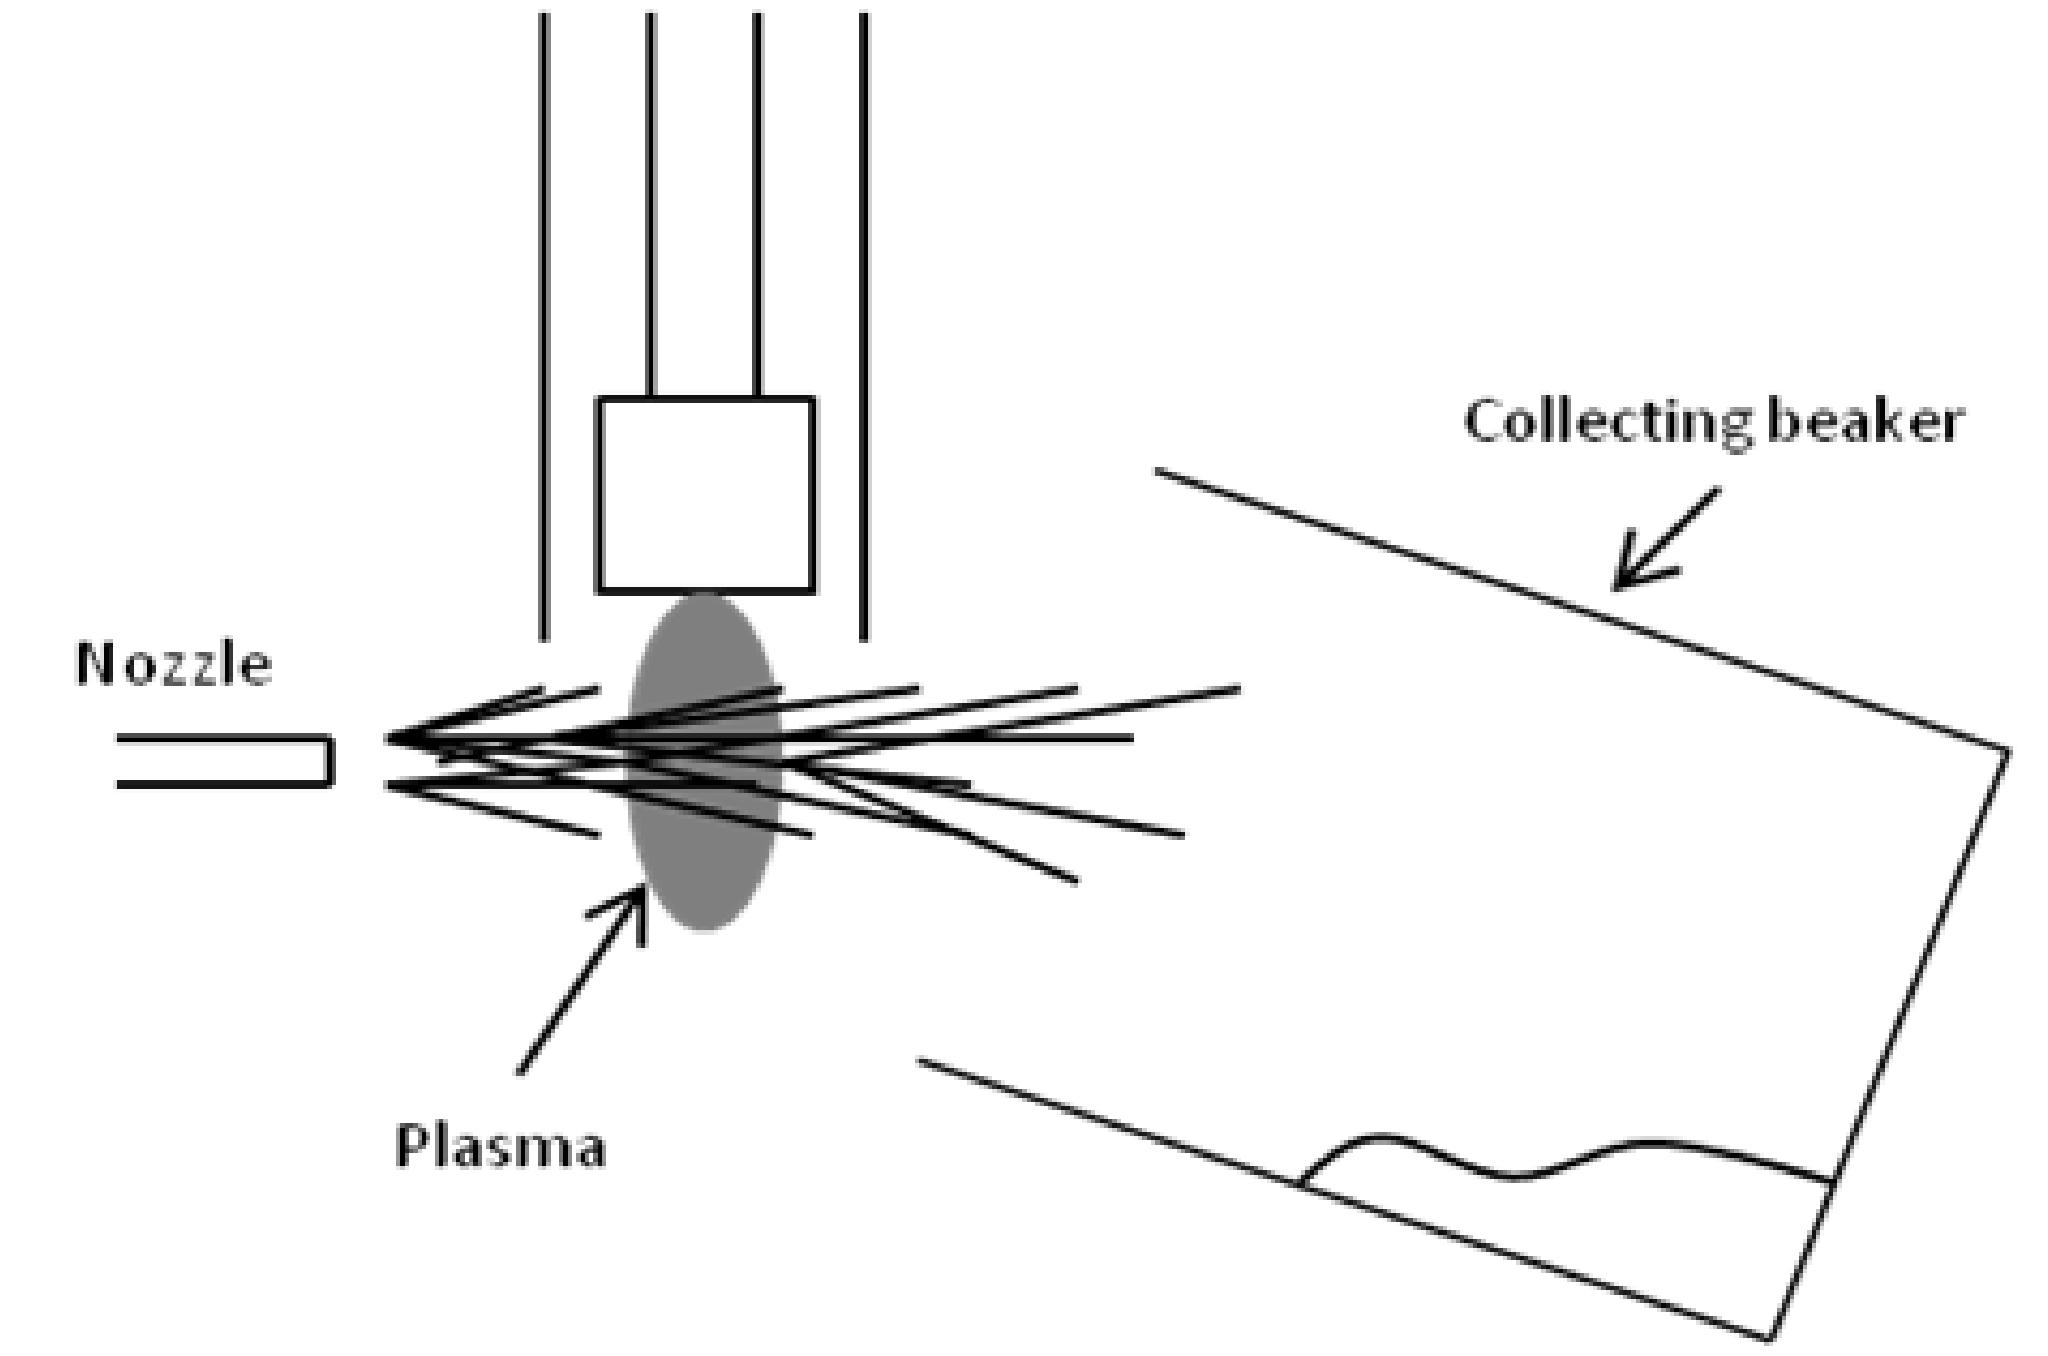
\includegraphics[width=0.9\textwidth]{Figure6_word.jpg}
  \caption{Set-up for introducing water directly into the active plasma region.  A greenhouse sprayer injects water from the side of the plasma source; water is collected in a beaker on the other side}
  \label{fig:spray_scheme}
\end{figure}

A comparison of batch and greenhouse sprayer configurations for generation of nitrate in solution per unit energy is shown in \cref{fig:nitro_compare_power}. It is found that in general the greenhouse sprayer configuration performs more favorably than the batch treatment design. This is especially clear at higher powers. Moreover, the performance of the greenhouse sprayer configuration appears to improve with increasing power delivered to the plasma. However, increasing plasma power also has some negative effects. One is an increased rate of erosion of the powered electrode. A second negative consequence is poorer matching of the load impedance resulting in increased reflected power back to the generator. Both of these effects decrease the lifetime of the design; decreasing the lifetime of the generator is particularly undesirable because of its cost.

Another issue with the greenhouse sprayer configuration that ultimately curtails further investigation is the instability of the plasma. The sprayer must be placed such that droplets do not touch the surface of the powered electrode or else the plasma is immediately extinguished. Moreoever, even if the sprayer is properly placed and the electrode is not wetted, the plasma actively trys to avoid the droplet stream. Typically even in the most optimized sprayer set-up, the plasma extinguishes after a few tens of seconds. Compare this with the batch set-up in which water can be treated continuously for multiple hours.

\subsection{Built-in Nozzle}

\section{Base electrode designs}

As mentioned in \cref{sec:spray_bottle}, plasma erosion of the source's powered electrode can occur, especially at higher powers. Evidence of this erosion can be seen both with the naked eye (see \cref{fig:OES_alum_damage}) and in the optical emission spectrum of the discharge. \Cref{fig:OES_alum_damage} shows the presence of an atomic aluminum line at 395 nm and several AlO bands between 425 and 575 nm. Visually, this emission manifests itself as an intense bright blue; an example of it can be seen in \cref{fig:diox_argon}.

\begin{figure}[htbp]
  \centering
  \includegraphics{damaged_aluminum_OES_spectrum.png}
  \caption{OES spectrum of plasma damaged aluminum electrode}
  \label{fig:OES_alum_damage}
\end{figure}

\begin{figure}[htbp]
  \centering
  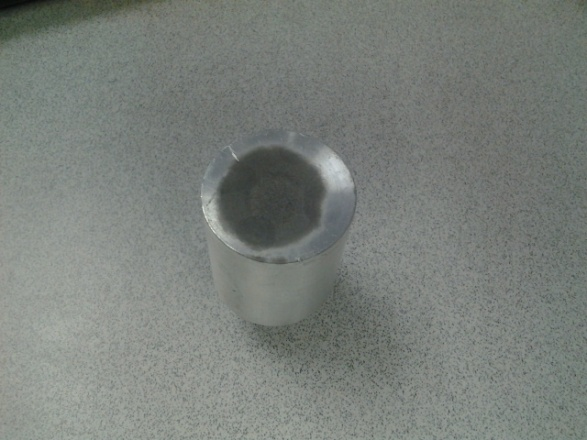
\includegraphics{full_size_alum_electrode_damage.jpg}
  \caption{Image of aluminum electrode after plasma erosion}
  \label{fig:alum_damage_full}
\end{figure}

The plasma damage to the electrode can be investigated more closely using Secondary Electron Microscopy (SEM) and Energy Dispersive X-ray Spectroscopy (EDS). Even with a 1mm zoom (\cref{fig:alum_damage_1mm}), the growth of a damage layer is evident. Taking an EDS measurement of the clean aluminum yields the spectrum shown in \cref{fig:EDS_clean_alum}. Unsurprisingly, the spectrum shows almost pure aluminum with a trace of magnesium. An EDS scan of the damaged aluminum portion, however, reveals the growth of substantial carbon and oxygen peaks (\cref{fig:EDS_damaged_alum}). The oxidation is unsurprising considering the flow gas is often compressed air and the ambient environment is also air (also consistent with the OES spectrum (\cref{fig:OES_alum_damage})). The carbon could be coming from oils/hydrocarbons present in the compressed air feed.

\begin{figure}[htbp]
  \centering
  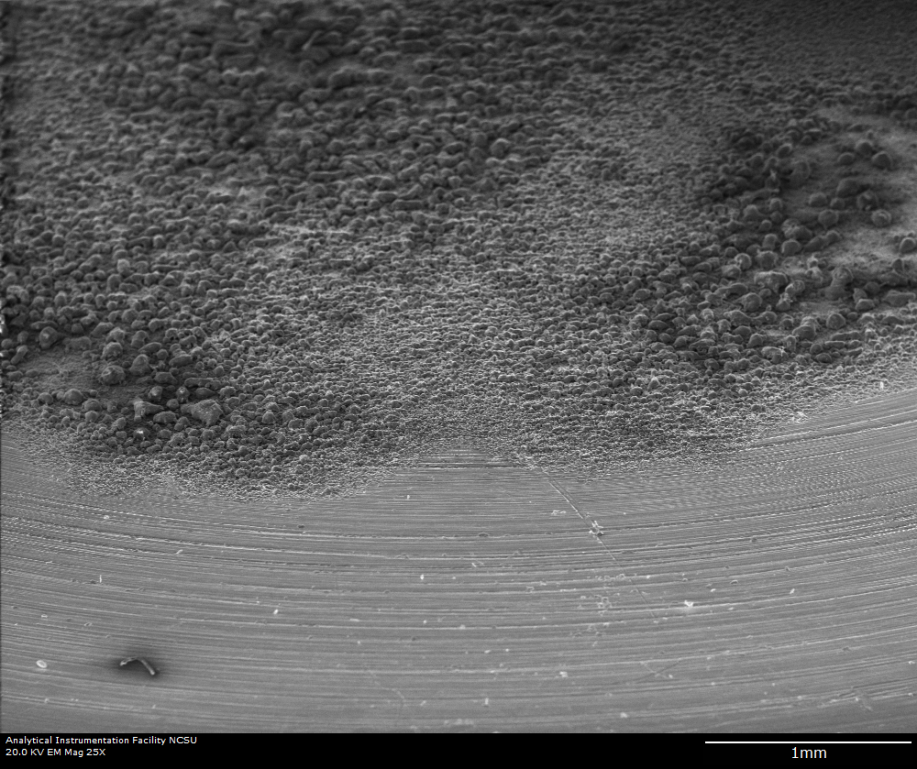
\includegraphics{1mm_zoom_tilt_alum_electrode_damage.png}
  \caption{SEM image of aluminum electrode after plasma erosion. 1mm zoom. 45 degree tilt.}
  \label{fig:alum_damage_1mm}
\end{figure}

\begin{figure}[htbp]
  \centering
  \includegraphics[width=0.9\textwidth, height=0.9\textheight, keepaspectratio]{clean_alum_eds.png}
  \caption{Energy dispersive X-ray spec (EDS) for clean aluminum electrode}
  \label{fig:EDS_clean_alum}
\end{figure}

\begin{figure}[htbp]
  \centering
  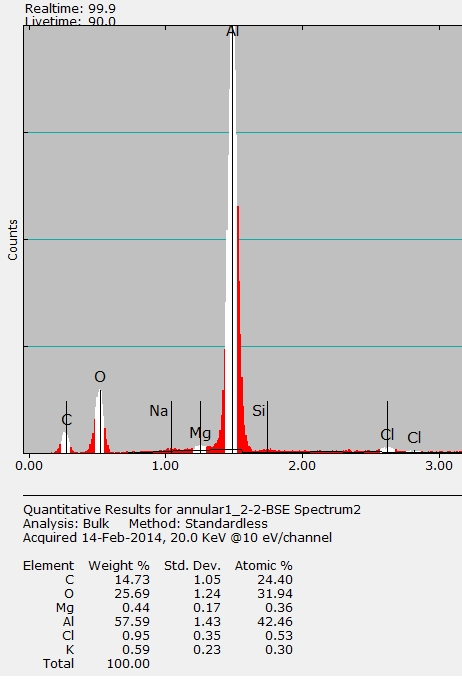
\includegraphics[width=0.9\textwidth, height=0.9\textheight, keepaspectratio]{damaged_alum_eds.png}
  \caption{Energy dispersive X-ray spec (EDS) for plasma eroded aluminum electrode}
  \label{fig:EDS_damaged_alum}
\end{figure}

In an attempt to prolong the lifetime of the powered electrode, metals other than aluminum are considered. A relatively inexpensive choice is brass. Overall brass performs much better than aluminum. Between 300-700 W, there is no plasma-metal interactions observed with OES or presence of pitting when the plasma is turned off. Typically aluminum begins to erode around 560 W. When the brass electrode is run between 700-1000 W, plasma-metal interactions are evinced by a plasma color change as well as an increase in the intensity of the emitted light. A comparison of the plasma OES with and without metal interactions is shown in \cref{fig:OES_brass_damage}. The 560 W spectrum shows a more or less normal air plasma spectrum: NO bands between 230 and 290 nm (along with their 2x peaks around 500nm) and an OH band around 310 nm. However, the 945 W spectrum is dominated by sharp copper and zinc atomic lines. Despite the presence of copper and zinc in the discharge emission, no visual damage appears on the electrode surface when operated between 700 and 1000 W. Though if the power is raised too much over 1000 W, surface pitting and scarring analagous to the damage on the aluminum electrode is observed (see \cref{fig:brass_damage_full}).

\begin{figure}[htbp]
  \centering
  \includegraphics[width=0.9\textwidth]{damaged_brass.jpg}
  \caption{Image of brass electrode after plasma erosion}
  \label{fig:brass_damage_full}
\end{figure}

\begin{figure}[htbp]
  \centering
  \includegraphics{damaged_brass_OES_spectrum.png}
  \caption{OES spectrum of plasma damaged brass electrode}
  \label{fig:OES_brass_damage}
\end{figure}

\section{Water Electrodes}
\label{sec:water_electrodes}

An ideal plasma-liquid geometry has to provide both maximum interfacial contact between reactive plasma species and the liquid phase as well as parts that are resistent to plasma corrosion. Unfortunately, none of our previous configurations realize this goal. However, by utilizing the unique nature of the VHF source and recognizing the fact that the entire coaxial structure is DC grounded, we can do something rather novel. We can apply a liquid layer to the surface of the powered electrode without worry of causing a short circuit. With this configuration, shown in \cref{fig:water_electrode_scheme}, the treated water is exposed to the most reactive part of the plasma. Both ion and electron fluxes to the water surface are anticipated to be much higher than in the batch configuration. Additionally, powered plasma-facing solid surfaces are completely eliminated from the geometry. The liquid surface is forever renewable. This reduces system cost as well as experimental down-time.

\begin{figure}[htbp]
  \centering
  \includegraphics[width=0.9\textwidth]{water_electrode_geometry.png}
  \caption{Representative experimental set-up for using a ``water'' electrode}
  \label{fig:water_electrode_scheme}
\end{figure}

The actual design of the water electrode can be seen in \cref{fig:water_electrodes_image}. The electrode of most utility, the ``pure'' water electrode, is shown on the right. The pure water electrode has no powered metal surfaces; the powered surface is 100\% water. If some plasma-metal contact is desired, for instance if that contact favorably modifies some plasma or liquid application variable, then the ``annular'' electrode shown on the left can be used.

\begin{figure}[htbp]
  \centering
  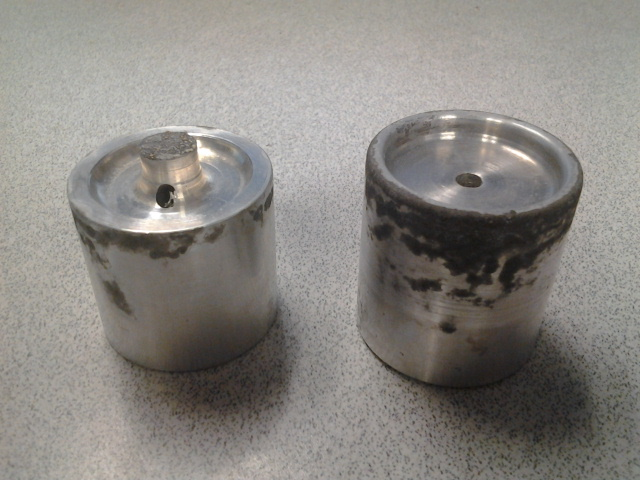
\includegraphics[width=0.9\textwidth]{water_and_annular_electrodes.jpg}
  \caption{Image of the two versions of ``water'' electrodes. The ``annular'' version still allows a small metallic area of plasma contact. In the ``pure'' version, the plasma has no metallic content with the powered electrode. The powered surface is entirely composed of water.}
  \label{fig:water_electrodes_image}
\end{figure}

\Cref{fig:annular_vs_water_oes} compares stereotypical OES spectra obtained for annular and pure water electrodes running at 700 W. Evidence of plasma-metal contact with the annular electrode is evident in the presence of aluminum atomic lines and AlO molecular bands. Additionally, there is a sodium line from sputtering of the tap water. The pure water electrode spectrum is much less intense and consists only of OH bands.

\begin{figure}[htbp]
  \centering
  \includegraphics{annular_vs_water_electrode_oes.png}
  \caption{Comparison of OES spectra for annular and pure water electrodes}
  \label{fig:annular_vs_water_oes}
\end{figure}

\Cref{fig:pow_sweep_water} shows the effect of increasing power on the optical emission spectrum with the pure water electrode. Because the plasma is in immediate contact with the water surface and not any solid surfaces, the device can be operated at much higher powers. Whereas with a metal electrode the source cannot be run at powers much greater than 700 W without significant damage to the electrode, the pure water electrode can be run up to 1155 W. The only reason that the device cannot be operated at even higher powers is because of the increased difficulty in matching impedances using the main and stub lines; reflected power becomes high enough to damage the generator.

Up above 1000 W, aluminum atomic lines and AlO bands become apparent (\cref{fig:pow_sweep_water}. The presence of the aluminum associated emissions is interesting because the metal is removed from the gaseous discharge region by the few milimeter thick water layer; this probably explains why the intensities are significantly below that of discharges with direct plasma-metal contact (see \cref{fig:annular_vs_water_oes}). However, the existence of any aluminum lines at all implies that the discharge is penetrating the aqueous phase to reach the metal. This is perhaps indirect evidence of high charged particle fluxes to the water electrode surface, suggesting that the pure water electrode design is a good one for maximizing interactions between the plasma and aqueous phases.

\begin{figure}[htbp]
  \centering
  \includegraphics{water_electrode_power_sweep_oes.png}
  \caption{OES spetra showing power sweep with pure water electrode. Relatively small aluminum peaks grow in at very high powers.}
  \label{fig:pow_sweep_water}
\end{figure}

% Note that there is a lot of OH rotational measurement as well as nitrite and nitrate concentration measurements for the water electrodes that are in my ICOPS 2014 presentation. I think the data looks like a bunch of garbage with no clear trends so I'm omitting it for now. However, if I need more material, I can perhaps come back to it.

\subsection{Early Absorption Work}

% Waiting on some figures from Brandon
